% Chapter 4

\chapter{Data, Methods, and Implementation} % Main chapter title

\label{Chapter4} % For referencing the chapter elsewhere, use \ref{Chapter1} 

\lhead{Chapter 4. \emph{Data, Methods, and Implementation}} % This is for the header on each page - perhaps a shortened title

\emph{This chapter presents the different strands of our work. The work is divided into three components: first, the procurement of HEP training data on which to perform experiments; the implementations of extensions to GROBID to facilitate the feature engineering and evaluations, as well as the pipeline assembled for automating the experimentation; and finally, the different categories of feature engineering, and our reasons for choosing them, supplying, where relevant, statistical analyses to support our intuitions.}

\section{Assessments}

As articulated in Chapter \ref{Chapter3}, GROBID manages a hierarchy of models that propagates classified information from top to bottom in a cascade. Our objectives are therefore to enhance some models within the cascade for HEP papers. It does not, on the other hand, make sense to attempt to improve all models. After all, we may assume a HEP \emph{date} is no different from dates printed in other scientific papers.The same goes for author names, and with little exception\footnote{It is in fact true that HEP collaborations feature in isolated references in HEP papers (see Section \ref{sec:futurework}).}, reference lists and their contents. Undoubtedly, the models with the most promising scope for improvement are the \emph{header} and \emph{segmentation} models. It is these models that address the parts of an article most distinct in scientific papers. Specifically, physics journals have recurring styles and layouts for headers sections that are distinct from others publishers. In addition, the vocabulary of a HEP paper header will be distinct from that of papers from other branches of science. These should be both trained for and engineered for, for example through the use of dictionary-based features (see Section \ref{subsec:dicts}). Exceptionally, the \emph{header} model is not, by default, part of the cascade, rather, the header section is extracted separately using heuristics based on locating the start of the body (usually identified by the heading, `Introduction'). The reason for this approach is that, on average, it is more accurate than relying on the \emph{segmentation} model for finding front matter, given the limited amount of \emph{segmentation} training data. However, this precludes the modelling of \emph{discontinuous} front matter, which may occur at the base of a first page, at the very end of an article, or just about anywhere else (see Figure \ref{fig:articlesamples}). Reconnecting the \emph{header} model with with the \emph{segmentation} model is therefore an implementation objective. Thus, the \emph{header} model may be improved for a number of reasons, including:

\begin{enumerate}
\item physics publishers present a unique format not found in CORA papers;
\item scientific collaborations as seen in HEP papers are not modelled as a header class by vanilla GROBID, and;
\item discontinuous header data (see Figure \ref{fig:articlesamples}), which may contain substantial front matter is by default neither trained nor modelled for.
\end{enumerate}

The \emph{segmentation} model may also be improved for a number of reasons:

\begin{enumerate}
\item discontinuous header data (see Figure \ref{fig:articlesamples}), which may contain substantial front matter is neither trained nor modelled for;
\item HEP collaborations entail long author lists and affiliation lists, often disjoint from the main header section, which are neither trained nor modelled for, and;
\item the dataset is small (we more than double it in Section \ref{sec:data}).
\end{enumerate}

Note that the \emph{segmentation} model is the parent model of the entire cascade, and therefore any improvement to it will benefit all other models at prediction time. Aside from being the root of the cascade, the \emph{segmentation} model is special in that it models a full line at the token level, rather than a single character string such as for the \emph{header} model. We are mindful of this distinction as we go about our feature engineering. Our focus is therefore on the two models, \emph{header} and \emph{segmentation}. Hence, we require two separate training sets of HEP papers. Both models require that for each paper we produce a TEI representation and a feature file of extracted features, as introduced in Section \ref{sec:grobid}.

\begin{figure}[b]
\centering
\begin{tabular}{cc}
\subfloat[Collaboration field in header section.]{
\includegraphics[width=0.45\textwidth]{Figures/collaboration.pdf}}\label{fig:articlesamplesA}&
\subfloat[Discontinuous header data.]{
\includegraphics[width=0.45\textwidth]{Figures/eamonn.pdf}} \\
\subfloat[Collaboration author list.]{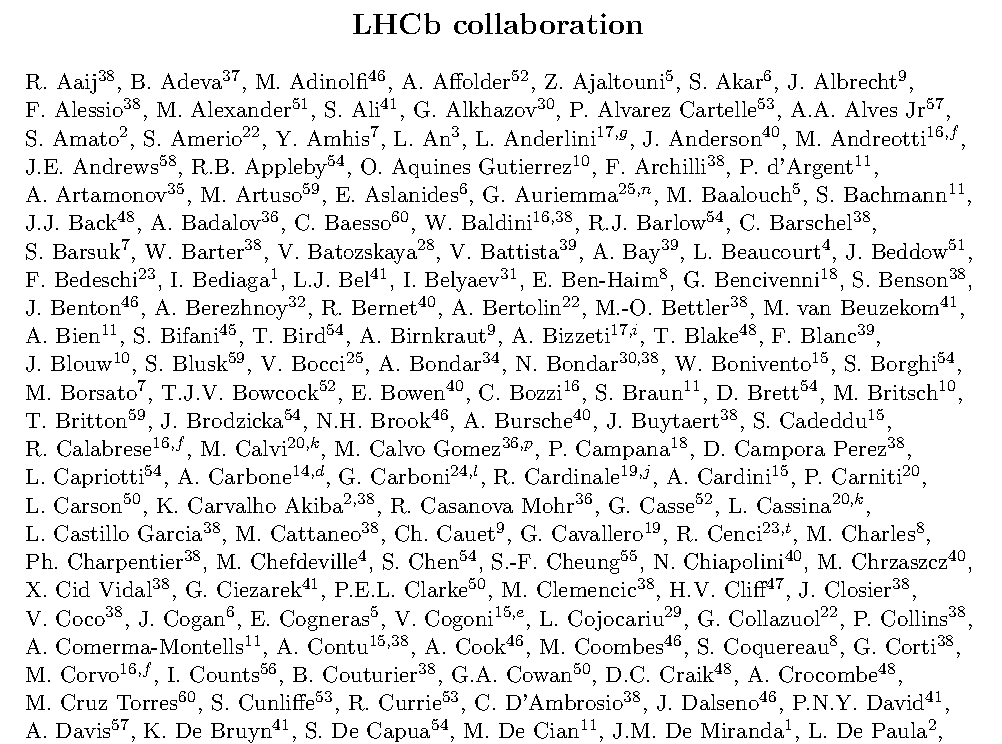
\includegraphics[width=0.45\textwidth]{Figures/authors.pdf}} & 
\subfloat[Collaboration affiliation list.]{
\includegraphics[width=0.45\textwidth]{Figures/affiliations.pdf}}\\
\end{tabular}
\caption{Figure (A) shows a collaboration field in a header section. Figure (B) shows discontinuous front matter that sits on the first page, but apart from the main header section and within the introductory section. Figures (C) and (D) give the authors list and affiliations for a large HEP collaboration; the author list begins on page 8 and continues to page 33. Figure (B) from (\cite{maguire2012taxonomy}), other excerpts from (\cite{aaij2015identification}).}
\label{fig:articlesamples}
\end{figure}

% \begin{table}[b]
% \begin{center} 
% \begin{tabular}{|c|c|c|}
% \hline
% Model & Token & Instance \\
% \hline
% Header & Character string & Header section \\
% \hline
% Segmentation & Full line & Full document \\
% \hline
% \end{tabular}
% \caption[Comparison of token and instance entities for \emph{header} and \emph{segmentation} models. For information on \emph{fields} tagged by these models, see Section \ref{sec:grobid}.]{Evaluation results for reference segmentation}
% \label{table:headervssegmentation}
% \end{center}
% \end{table}

\section{Data Acquisition}
\label{sec:data}

The starting point for generating training data is to apply the existing, shipped models of GROBID on our new dataset of PDF papers. This creates a pair of TEI and feature file for each document, in a first attempt at a ground truth, and a structure on which to work. Though this is greatly preferable to starting from scratch, researcher must then manually correct the inevitable myriad errors to achieve a gold standard of training data. In the case of \emph{segmentation}, this involves the validation of a full document, which may contain many recurring misclassifications, rendering the task stupendously time-consuming and a barrier to actual research. In the case of the \emph{header} model, this is often simpler, as it involves validating a single section. However, wherever discontinuous front matter exists, changes must be made to both the TEI \emph{and} feature files. This first involves a modification to GROBID such that it extract features for all tokens rather than just those contained in the header. Then, the unseen front matter must be manually formatted and appended to the TEI file, and the corresponding features copied to the feature file. This is error-prone, as there must be a one-to-one correspondence between the token in the TEI file and the features in the feature file. Hence, any copyist mistake will invoke errors at training time. In Sections \ref{subsec:cora}, \ref{subsec:hepdataset}, we detail the mixture of training data that we have assembled. Table \ref{table:hepvscora} gives a breakdown of the data for each model.

\begin{table}[h]
\begin{center}
\begin{tabular}{|c|c|c|}
\hline
Model & HEP & CORA \\
\hline
Header & 157 papers & \textbf{2506 papers} \\
\hline
Segmentation & \textbf{169 papers} & 125 papers \\
\hline
\end{tabular}
\caption[Number of training instances for each model from each dataset.]{Number of training instances for each model from each dataset.}
\label{table:hepvscora}
\end{center}
\end{table}

\subsection{CORA dataset}
\label{subsec:cora}
The CORA dataset (\cite{mccallum2000automating}) is a substantial dataset of annotated documents. It is popular in metadata extraction studies, and has come to be a sort of standard due to the difficulty of creating custom data (\cite{Peng04accurateinformation}). We use it in combination with our own HEP dataset. For the \emph{segmentation} model, the baseline dataset is not part of CORA, but rather part of the GROBID project, but for brevity we refer to this also as \emph{CORA}.

\subsection{HEP dataset}
\label{subsec:hepdataset}

At the recommendation of an INSPIRE-HEP digital library curator, we selected a set of articles deemed to be a representative sample of the database. It contains the following varieties of papers:

\begin{enumerate}
\item conference papers (with DOI);
\item conference papers (without DOI);
\item miscellaneous papers (including non-English language), and;
\item collaboration papers.
\item general papers;
\end{enumerate}

This totalled 191 papers\footnote{Originally this numbered in excess of 200, but certain papers could not be parsed by \emph{pdf2xml}.}, however according to our adjudications, we additionally removed documents found to be unsuitable for training, such as books-length article compendiums. To start creating HEP \emph{header} model training data, we execute GROBID command, \texttt{createTrainingHeader}. Modifications were made to GROBID to produce header features for an entire document, rather than just the first two pages as per the default. This was essential in order to obtain features for any discontinuous front matter in other parts of a document. Wherever such matter was found, it was necessary first to manually append this material to the TEI file, following the TEI XML standard, then to copy the discontinuous segments of the extracted features into the master copy feature file. Whenever a copyist mistake was made, this entailed runtime errors, and lengthy corrections. For \emph{segmentation} training data, we run command \texttt{createTrainingSegmentation}. The starting point for building a \emph{segmentation} training set is invariably worse than for \emph{header}, due to the lower accuracy of this model. Typically each instance contains many recurrent misclassifications which sometimes may be corrected efficiently using regular expressions.

% Therefore one of our research questions is whether such a mixture is beneficial, and we experiment with different CORA sample sizes in Chapter \ref{Chapter5}.

\section{Methods}
\label{sec:featurengineering}

Here we list the ideas for feature functions that we have implemented and cross-validate for in Chapter \ref{Chapter5}. The features were extracted either with changes made to GROBID directly, or by modifying baseline features with an external script from our pipeline (Section \ref{subsec:pipeline}). In the following we use a notation consistent with that introduced in Chapter \ref{Chapter2}, that is, $x$ represents a token, $\mathbf{x}$ an instance, and $y$ and $\textbf{y}$ the corresponding label and label vectors. 

% Where discretisation is necessary, we first present the unaltered numeric feature function, $\hat f(\cdot)$, then its discretised version, $f(\cdot) = \lfloor C \cdot \hat f(\cdot)\rfloor$, where $C$ is some discretisation factor assigning the floating point values to $C$ bins.

\subsection{Baseline}

To set a benchmark by which to compare our results, we ran a series of experiments including the default features for GROBID, training on different combinations of CORA and HEP data (see Section \ref{sec:experimentsetup}). In addition, we examined the effects of ramping up the size of the CORA set appended during training. Baseline features include token identities, prefixes, suffixes, and indicators of capitalisation, numerals, and so on. Our new features were combined with the baseline features unless otherwise noted.

\subsection{Block Size}

A block is a collection of lines physically grouped together. The block to which each token belongs is specified in the \emph{pdftoxml} outputs. One characteristic that is distinct about article layout are the varied dimensions of blocks. This is most striking in the header section, where different blocks manifest in distinct sizes. For example, an article title is usually wider than any other element, an abstract is the longest element, and so on. It seems reasonable that the dimensions of a block to which a token belongs may provide information on the class of the token. We therefore devise features based on the pixel lengths and widths of header text blocks, information that comes from \emph{pdftoxml}. We try four variations on this idea: block width, block height, block width and height together, and block area, each normalised by the largest block dimensions. For example, for area, the feature function is,

\begin{equation}
\hat f_{size}(x_t) = \frac{\sum_{b \in B} \mathbbm{1}_{\{x_t \in b\}} \cdot\text{height}(b)\cdot\text{width}(b)}{\text{max}_{b' \in B} \text{height}(b') \cdot \text{max}_{b'' \in B} \text{width}(b'')},
\label{eq:areafunction}
\end{equation}

where $x_t$ is a token (hence a word for the \emph{header} model) and $B$ is the set of blocks in the header instance. We then define,

\begin{equation}
f_{size}(x_t) = \big\lfloor C \cdot\hat f_{size}(x_t)\big\rfloor,
\label{eq:areafunctiondisc}
\end{equation}

where $C$ is a discretisation factor. In our experiments $C = 10$, giving a categorical variable of 10 values.

\subsection{Character Classes}
\label{subsec:characterclasses}
A visual scan of any scientific paper allows one to see that lines from different sections are most easily distinguished by their composition of characters. It therefore stands to reason that we can build informative features for the \emph{segmentation} model on this basis. Indeed, it can be that a line may be more effectively characterised at the \emph{character} level than the \emph{word} level. For an illustration of this effect, see Figure \ref{fig:radar}. Note that the baseline feature function set does include some basic capitalisation and punctuation indicators, but we advocate our approach for several reasons:

\begin{enumerate}
\item it is more complete in that it models more character classes;
\item it does this systematically in a feature framework that is easily modified or extended, and;
\item it performs better (see Chapter \ref{Chapter5}).
\end{enumerate}

In Table \ref{table:characterclasses}, we give a list of the character classes used to model features. The regular expressions (regexes) were used to count the number  of characters in a token (line) belonging to each class. This was then normalised over the line length. Because such a result is numeric, we have necessarily to discretise it. We tried four different discretisation strategies: binary (according to some \emph{ad hoc} threshold), decimal (round down), decimal (round to nearest), and 20-point discretisation\footnote{In this final discretisation case we categorised results by each $5th$ percentage point, capping at $50\%$, such that we model 10 categories in total.}. For the decimal case (rounding down),

\begin{equation}
\hat f_{\text{class}_i}(x_t) = \frac{1}{|x_t|}\sum_{n=1}^{|x_t|} \mathbbm{1}_{\{x_{ti} \in \text{class}_i\}},
\label{eq:classfunctions}
\end{equation}

for each character class, $\text{class}_i$, where $x_t$ is a token (hence a line for the \emph{segmentation} model), and $x_{ti}$ is the $ith$ character in the line. For the decimal (round down) case, we then define,

\begin{equation}
f_{\text{class}_i}(x_t) = \big\lfloor C \cdot\hat f_{\text{class}_i}(x_t)\big\rfloor,
\label{eq:classfunctionsdisc}
\end{equation}

where $C$ is the discretisation factor and $C = 10$. The other discretisation strategies may be defined similarly.

\begin{table}[h]
\begin{center}
\begin{tabular}{|c|l|l|}
\hline
Class & Regex\\
\hline
Spacing & r`[\textbackslash s]'\\
Lower case & r`[a-z]'\\
Upper case & r`[A-Z]'\\
Numeric & r`[\textbackslash d]'\\
Punctuation & r`[\(\).,?:;]'\\
Special character & r`[\^{}\textbackslash sa-zA-Z\ d\(\).,?:;]'\\
\hline
\end{tabular}
\caption[Character classes used as features, along with the regular expressions used to count them.]{Character classes used as features, along with the regular expressions used to count them.}
\label{table:characterclasses}
\end{center}
\end{table}

\begin{figure}
\centering
\begin{tabular}{cc}
\subfloat[Body (formula)]{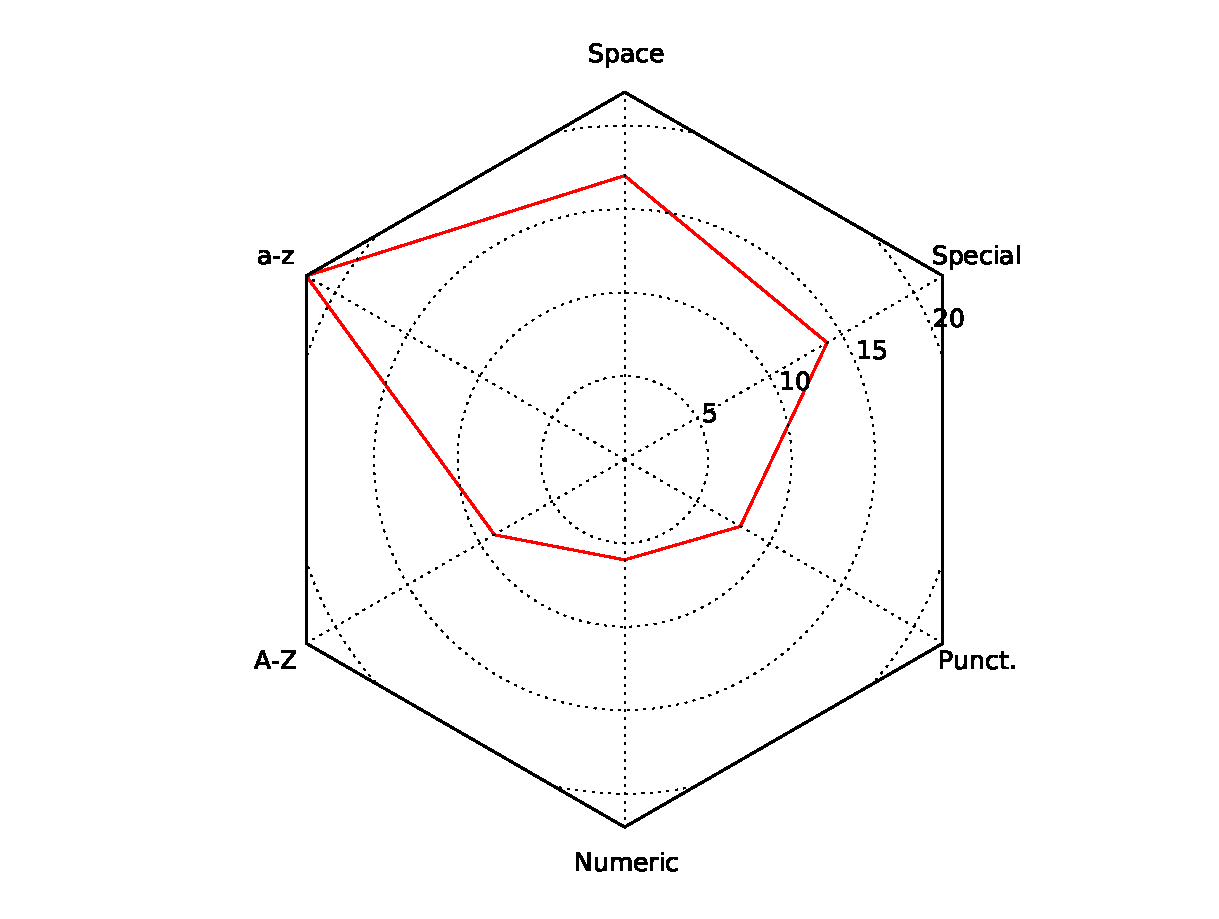
\includegraphics[width=0.5\textwidth]{Figures/body_formula.pdf}} & 
\subfloat[Body (normal)]{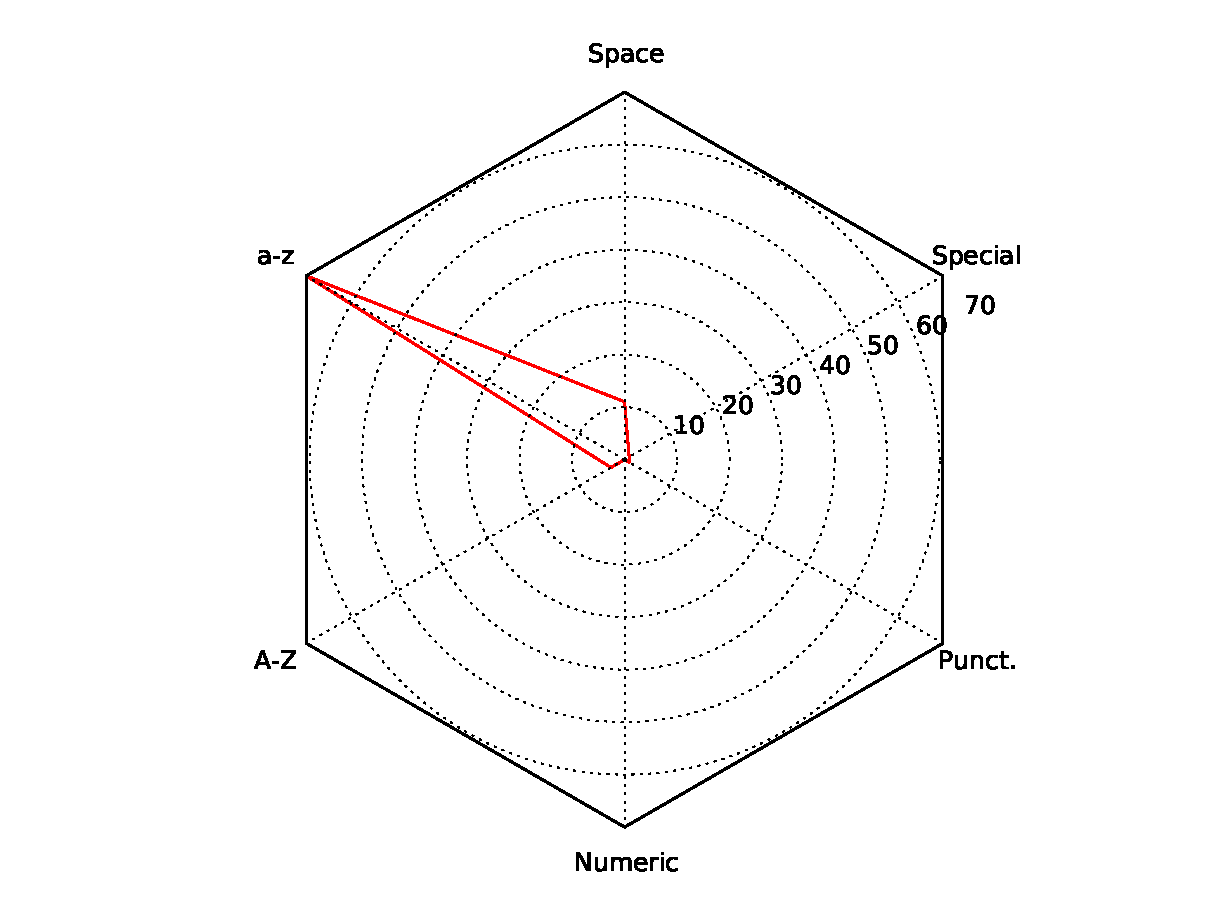
\includegraphics[width=0.5\textwidth]{Figures/body_normal.pdf}}\\
\subfloat[Headnote]{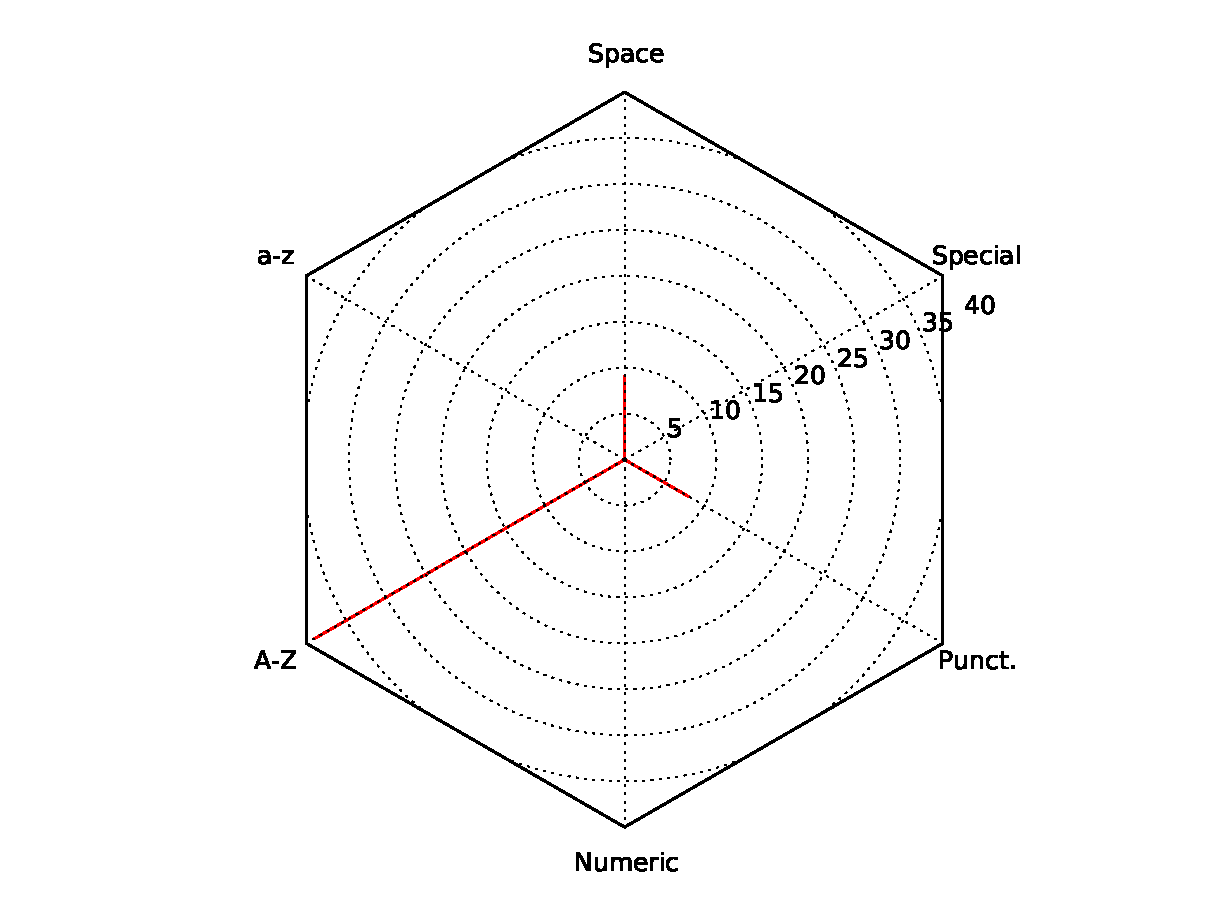
\includegraphics[width=0.5\textwidth]{Figures/headnote.pdf}}&
\subfloat[Page number]{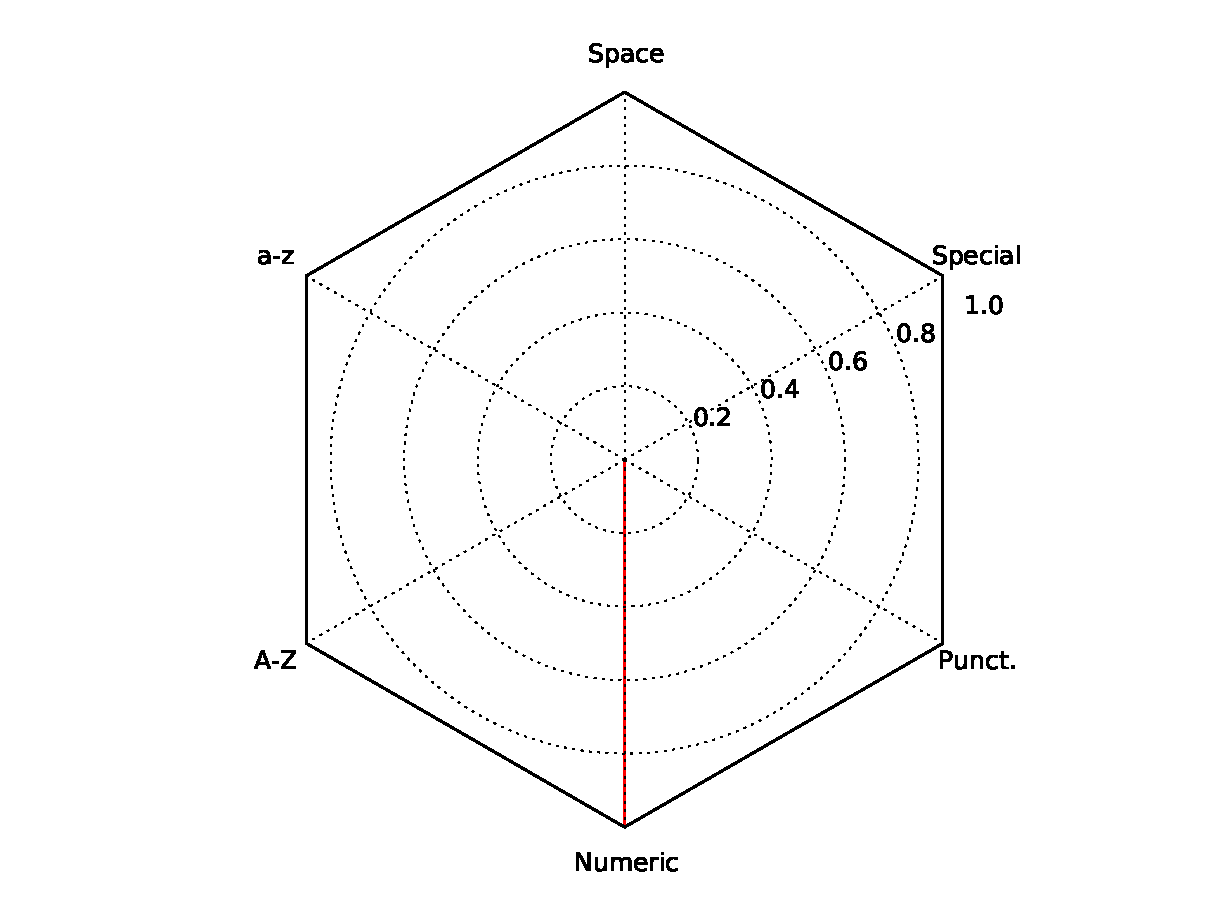
\includegraphics[width=0.5\textwidth]{Figures/page.pdf}} \\
\subfloat[Affilation list]{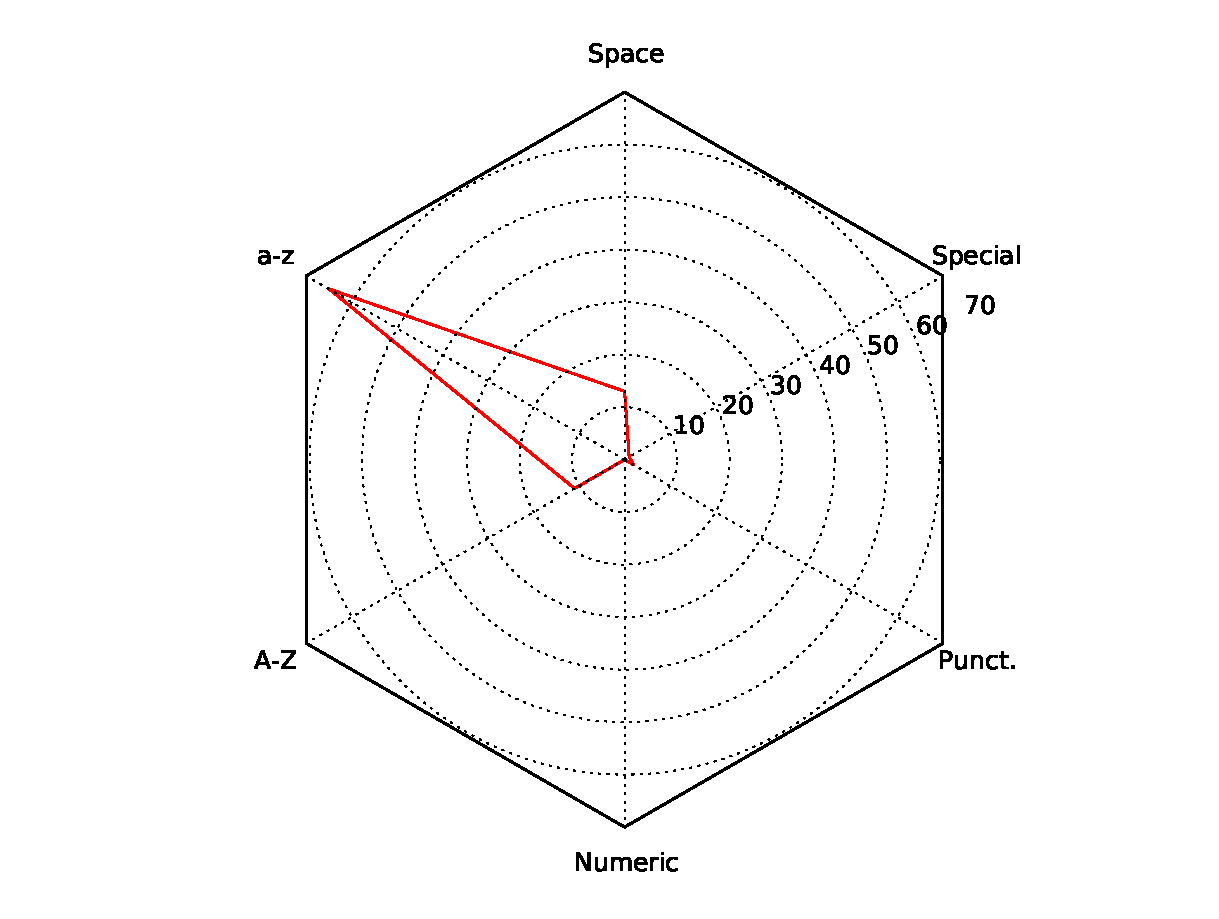
\includegraphics[width=0.5\textwidth]{Figures/affiliations_list.pdf}} & 
\subfloat[Author list]{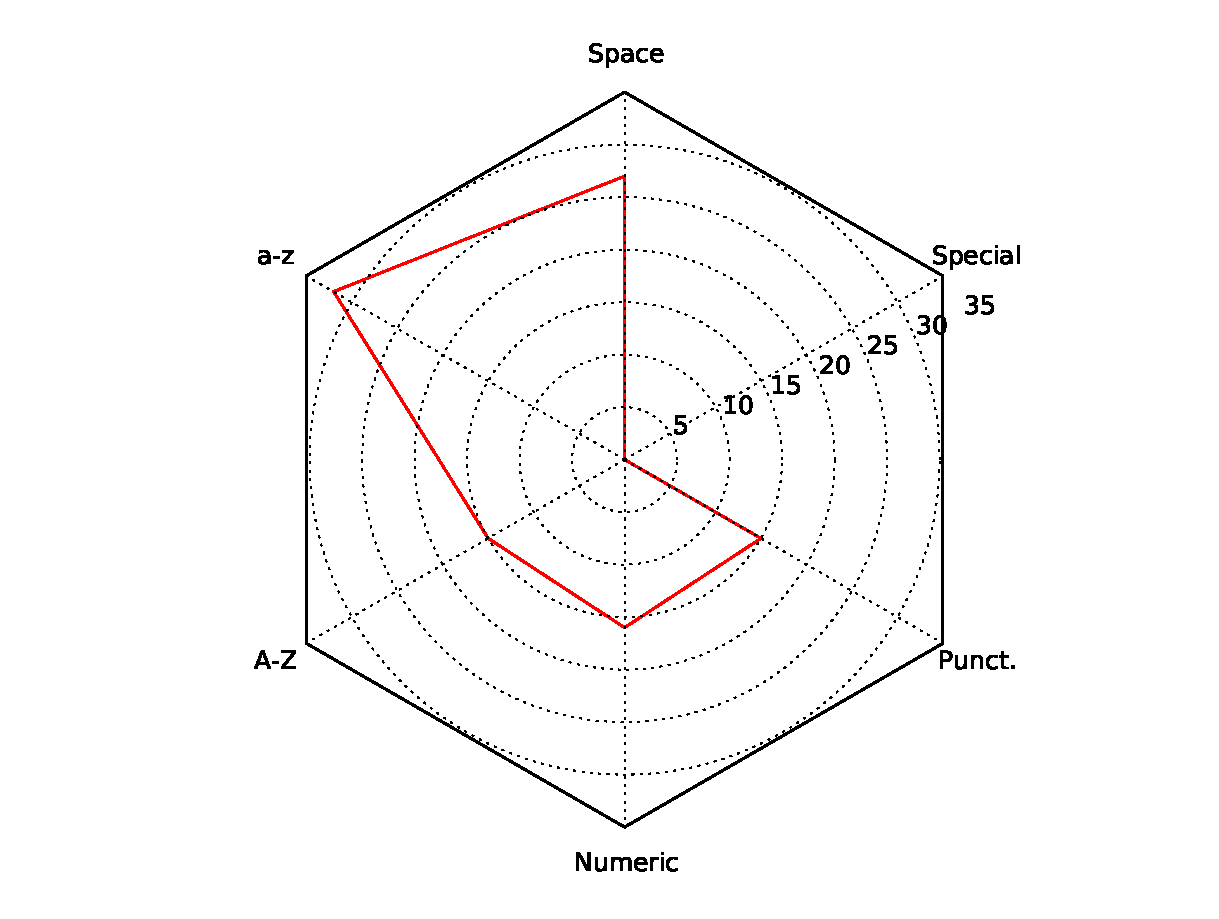
\includegraphics[width=0.5\textwidth]{Figures/author_list.pdf}} \\ 
\end{tabular}
\caption{Character class breakdown of sample lines from different sections of a CERN LHCb collaboration paper. The paper in question is the current world record holder for number of authors, and lists over 5000 authors and their affiliations. The radar plots give a different impression for each of the samples.}
\label{fig:radar}
\end{figure}

\subsection{Dictionaries}
\label{subsec:dicts}

As mentioned previously, the vocabulary of a HEP paper \emph{header} is distinct from other branches of science, containing jargon and terminology particular to high energy physics. Aside from token indicators, we can support this characteristic with features based on dictionary membership. To achieve this, we exported the full set of author names, affiliations, journal names, article titles, and collaborations from the INSPIRE-HEP database. These dictionaries were then tokenised to give a set of \emph{words} rather than phrases. Each dictionary required extensive cleaning prior to being fit for purpose. In addition, we used the Natural Language Toolkit (\texttt{nltk}) for Python to create a dictionary of stop words, the expectation being that different classes contain stop words in varying amounts. For example, prosaic text, such as an abstract, will contain stop words (the, a, an, it, etc.) in greater number than summary information such as a keyword term, or an author details block. We confirmed this hypothesis with statistical ANOVA and pairwise t-tests in $R$, showing significant differences of stop word frequency according to header section (see Appendix \ref{sec:stopwordfrequency}). The dictionary feature functions may therefore be written formally as,

\begin{equation}
f_{\text{dict}_i}(x_t) = \mathbbm{1}_{\{x_t \in \text{dict}_i\}},
\label{eq:classfunctions}
\end{equation}

for each dictionary, $\text{dict}_i$. These features did not require modifications to GROBID directly, and were instead created by editing baseline feature files with pipeline script, \texttt{feature\_modifier.py}.

\subsection{Levenshtein Distance}

The Levenshtein or \emph{edit} distance can be used to quantify the edit distance between two strings, $a$ and $b$, by counting the number of changes, insertions, or deletions required for transforming $a$ into $b$. Beginning with $\text{lev}_{a, b}(|a|, |b|)$, the recursive step is defined to be,

\begin{equation}
  \text{lev}_{a, b}(i, j) = 
  \begin{cases} 
  	\text{max}(i, j) &\quad\text{if min(i, j) = 0} \\
	\text{min}
		\begin{cases}
			\text{lev}_{a, b}(i - 1, j) + 1 \\
			\text{lev}_{a, b}(i, j - 1) + 1 \\
			\text{lev}_{a, b}(i - 1, j - 1) + 1_{a_i \neq b_j} \\
		\end{cases} &\quad\text{otherwise} \\
  \end{cases}
\label{eq:levenshtein}
\end{equation}

With some exploratory data analysis we may see that the average edit distance varies between different sections, in particular at the transition points between these sections. It therefore stands to reason that the Levenshtein distance may be used as a feature of line tokens in the \emph{segmentation} model. Therefore, we define a similarity measure based on the Levenshtein distance, first normalising the distance between a line and its precursor, by dividing by the length of the longer of the two, before subtracting this result from 1, to give a measure of similarity,

\begin{equation}
\text{similarity}(a, b) = 1 - \frac{\text{lev}_{a, b}(|a|, |b|)}{\text{max}(|a|, |b|)}.
\label{eq:levenshteinsimilarity}
\end{equation}

Due to the constraints on numeric features (see Section \ref{sec:wapiti}), we must discretise the result. Thus, for a given line, $x_t$, we define the feature function, 

\begin{equation}
  f_{lev}(x_t) =
  \begin{cases}
  	0 & \quad \text{if } 0 \leq \text{similarity}(x_t, x_{t-1}) \leq T_1 \\
	1 & \quad \text{if } T_1 \leq \text{similarity}(x_t, x_{t-1}) \leq T_2\\
	\vdots & \qquad \vdots \\
	$N-1$ & \quad \text{if } T_{N-1} \leq \text{similarity}(x_t, x_{t-1}) \leq 1 \\
  \end{cases}
\label{eq:levenshteinfunction}
\end{equation}

where $T_1, T_2, ..., T_{N-1}$ are thresholds selected to create the $N$ categories. We try several thresholding strategies in our experimentation (see Section \ref{sec:experimentsetup}).

\subsection{Regularisation}

We additionally cross-validated the tuning parameter for the model, the variance for $l_2$ regularisation, $\sigma^2$, for values on a logarithmic scale: $\sigma^2 = 0$, $\sigma^2 = \exp\{-6\}$, $\sigma^2 = \exp\{-5\}$\footnote{Wapiti default value.}, $\sigma^2 = \exp\{-4\}$, and $\sigma^2 = \exp\{-3\}$.
 % This tuning was performed on the HEP training data with the baseline feature set.

\subsection{Token Extensions}

In the baseline \emph{segmentation} model, only the first two words from each line are modelled as features. The model might therefore benefit from modelling more of the line. However, unlike character class features (Section \ref{subsec:characterclasses}), modelling the features and does not reduce the dimensionality of the model. The signal from these token extensions may therefore be too diffuse to make useful indicators. We nevertheless tried four variations on this idea, extending the feature set to model the first 5, 10, 15, and 20 words of each line.

\section{Implementation}
\subsection{Extensions to GROBID}
\label{subsec:extensions}

The effects of our extensions are seen in Sections \ref{subsec:pipeline}, \ref{sec:featurengineering} and finally in Chapter \ref{Chapter5} and wherever appropriate we indicate them. Extensions were made as a branch of GROBID in the following ways:

\begin{enumerate}
\item reconnecting the \emph{segmentation} and \emph{header} models;
\item modelling HEP specific header field, \emph{collaboration};
\item producing new features;
\item logging results automatically, and;
\item extending the evaluation utilities for our analysis and reporting aims.
\end{enumerate}

The most significant extension made was with the class, \texttt{ConfusionMatrix.java}, used within GROBID's \texttt{EvaluationUtilities.java} framework to create confusion matrix outputs, ultimately visualised by the pipeline (see Chapter \ref{Chapter5}). These allowed us to see which misclassifications were made most frequently. In addition, \texttt{ConfusionMatrix.java} tracks the documents on which the the model committed the most errors for each misclassification. A sample output is given in Figure \ref{fig:topk}. Modelling collaborations as a class of the \emph{header} model involved extending GROBID's training and tagging modules alike. An XML structure conforming to the TEI standard (Section \ref{subsec:tei}) was selected. An example of a successful prediction of a collaboration is given in Figure \ref{fig:collaboration}.

\begin{figure}[t]
\centering
\begin{BVerbatim}
(<header>, <body>)
	1343657.training.segmentation.tei.xml - 0.7292 (35)
	1342206.training.segmentation.tei.xml - 0.3571 (5)
	1345915.training.segmentation.tei.xml - 0.3333 (7)
	1344707.training.segmentation.tei.xml - 0.1765 (3)
	1347299.training.segmentation.tei.xml - 0.1667 (8)
\end{BVerbatim}
\caption{Misclassification of <header> to <body> proportion and count (given in parentheses) for five papers in an evaluation fold, an output of the confusion matrix utility.}
\label{fig:topk}
\end{figure}

\begin{figure}[t]
\lstset{language=XML}
\begin{lstlisting}
<author>
    <orgName>ALICE Collaboration</orgName>
</author>
\end{lstlisting}
\caption{Example of successfully classified collaboration. The choice of XML tags is ours and was selected to be consistent with the TEI standard.}
\label{fig:collaboration}
\end{figure}

\subsection{Experiment Pipeline}
\label{subsec:pipeline}

To automate the experimentation process, we developed a pipeline of scripts in Python, the language chosen for its ubiquity in INSPIRE-HEP. The repository is open source and hosted on GitHub\footnote{https://github.com/jcboyd/pykelet/src}. The pipeline begins with using GROBID (including all necessary extensions) to generate raw feature files for all TEI files in the ground truth dataset. These are then manually assembled into a stripped-down copy of GROBID (containing all necessary Java executables and additional data) and placed in directory, \texttt{batches/}, with other scenarios. The assemblage of training data depends on the data scenario desired. If we wish to cross-validate over all data, we simply ensure that both the \texttt{training/} and \texttt{evaluation/} directories within the GROBID project contain all the feature files, and that all TEI files are in \texttt{training/}. The cross validation (CV) process will move a fold from the training directory to the evaluation directory, and return it when the iteration is complete. If, however, we wish to \emph{append} data for training, yet exclude it from CV and evaluation, we place the features files only under \texttt{training/}. The process will then cross-validate only on those files present in \texttt{evaluation/}. GROBID requires both TEI and feature files to be present or else they are ignored. This trick allows us to run such complex experiments without modifying GROBID or its directory structure. Each iteration of CV produces a log file of results exported from GROBID's evaluation utilities. Another script then aggregates the file contents (token- and field-level performance metrics and confusion matrices) and visualises them automatically. The pipeline process is depicted in Figure \ref{fig:pipeline}. The pipeline consists of a Python wrapper for GROBID, \texttt{grobid.py}, written using \texttt{pyjnius}, a Python library for the manipulation of Java executables through the Java Native Interface (JNI)\footnote{Certain limitations on this led us to write a simpler Python \texttt{subprocess}-based wrapper also.}. For an iteration of CV, (\texttt{k\_fold\_cross\_validation.py}), our wrapper may be used in the following way:\\

\begin{lstlisting}[language=python, caption=Excerpt from our Python wrapper for GROBID, label={lst:grobid}]
grobid_trainer = GrobidTrainer(classpath=classpath_trainer,
                               grobid_home=grobid_home)
grobid_trainer.train(model)
grobid_trainer.evaluate(model)
\end{lstlisting}

The process uses Python scientific computing library, \texttt{numpy}, to randomly shuffle training data (according to a fixed seed), and then Python machine learning library \texttt{scikit-learn} to create CV folds. The folds are withheld during training and are evaluated upon in the conventional way. The output of CV is a set of log files containing results. These results are processed by further scripts to produce visualisations of confusion matrices and performance metric comparisons.

\begin{figure}[!ht]
\center
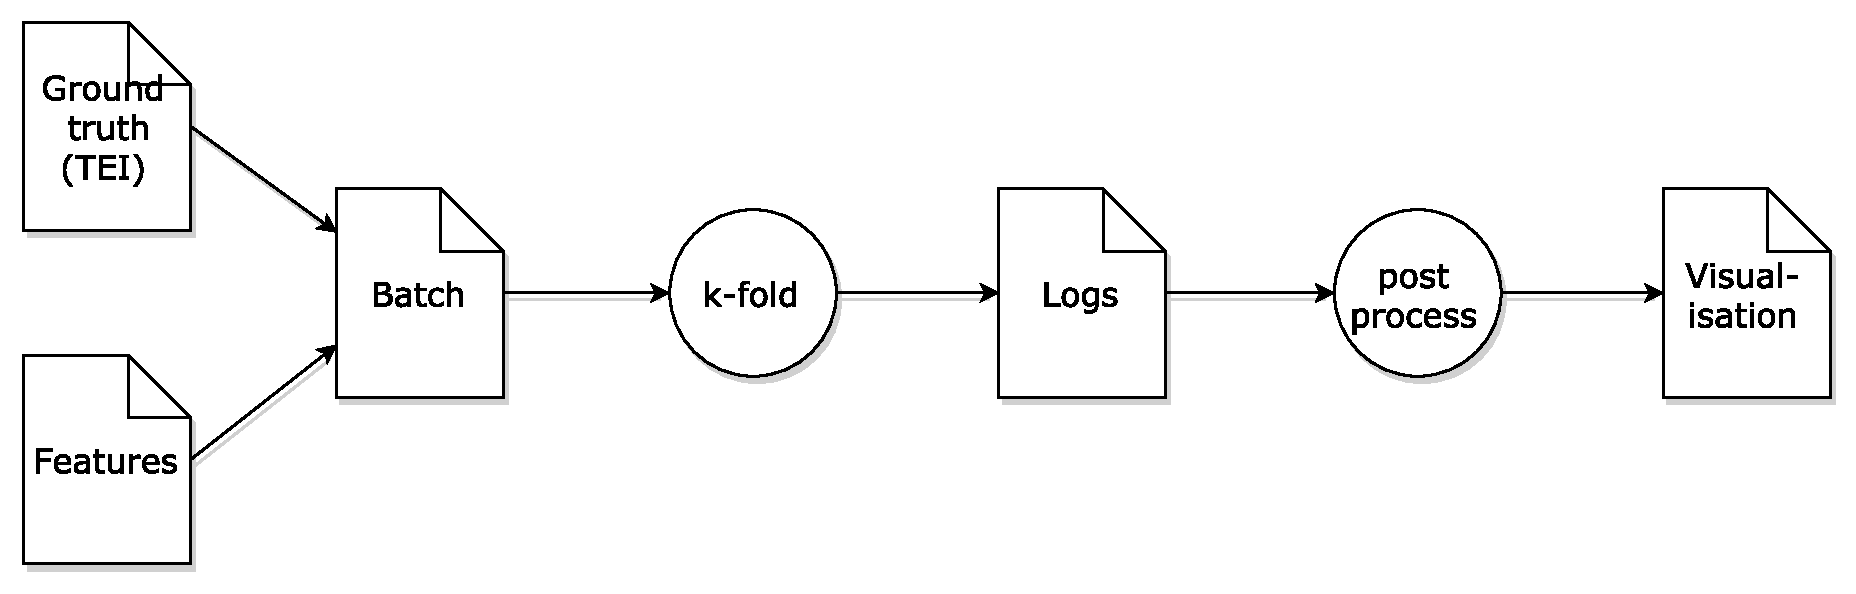
\includegraphics[width=\textwidth]{Figures/pipeline.pdf}
\caption{An illustration of the experimentation pipeline.}
\label{fig:pipeline}
\end{figure}
